\documentclass[12pt]{article}
\usepackage[utf8]{inputenc}
\usepackage[russian]{babel}
\usepackage{amssymb}
\usepackage{amsmath}
\usepackage{mathrsfs}
\usepackage{esvect}
\usepackage[left=2cm, right=2cm, top=2cm, bottom=2cm,
    bindingoffset=0cm]{geometry}
\usepackage[colorlinks=true, urlcolor=blue, linkcolor=blue, citecolor=blue,
    pdfborder={0 0 0}]{hyperref}
\usepackage{enumitem}
\usepackage{algorithm}
\usepackage{algpseudocode}

\hypersetup{frenchlinks=true}

\usepackage{graphicx}
\graphicspath{ {images/} }

\newtheorem{theorem}{Theorem}[section]
\newtheorem{lemma}[theorem]{Лемма}
\newtheorem{proposition}[theorem]{Предложение}
\newtheorem{remark}[theorem]{Замечание}
\newtheorem{corollary}[theorem]{Следствие}
\newtheorem{definition}[theorem]{Определение}
\newtheorem{example}[theorem]{Пример}

\newenvironment{proof}{\par $\triangleleft$}{$\triangleright$}

\pagestyle{plain}

\begin{document}

\begin{center}

    \Large \textbf{Фильтр Калмана}\\[0.5cm]
    \footnotesize {Немеш Н. Т.}\\[0.5cm]

\end{center}
\date{April 2022}

\section{Динамические системы}
\label{SectionDynamicSystems}

Существует много определений динамической системы. Мы будем рассматривать
непрерывные и дискретные нелинейные динамические системы с неаддитивным шумом. 
Данная заметка основана на статье \cite{QuatKinESKF}.

\subsection{Непрерывный случай}
\label{SubsectionContinuousCase}

\begin{definition}
    Динамической системой называется набор из вектор-функций нескольких переменных
    \begin{equation}
        \begin{aligned}
            f & :\mathbb{R}\times\mathbb{R}^n\times \mathbb{R}^m\times \mathbb{R}^p\to\mathbb{R}^n \\
            h & :\mathbb{R}\times\mathbb{R}^n\times\mathbb{R}^q\to\mathbb{R}^l                     \\
        \end{aligned}
    \end{equation}
    векторнозначных случайных процессов (функций со значениями в случайных векторах)
    \begin{equation}
        \begin{aligned}
            \pmb{x}:\mathbb{R}\to\mathbb{R}^n \qquad
            \pmb{z}:\mathbb{R}\to\mathbb{R}^l \qquad
            \pmb{\mu}:\mathbb{R}\to\mathbb{R}^q \qquad
            \pmb{\nu}:\mathbb{R}\to\mathbb{R}^p \qquad
        \end{aligned}
    \end{equation}
    и одной вектор-функции
    \begin{equation}
        \begin{aligned}
            u:\mathbb{R}\to\mathbb{R}^m
        \end{aligned}
    \end{equation}
    таких, что
    \begin{equation}
        \frac{d \pmb{x}(t)}{dt}=f(t, \pmb{x}(t), u(t), \pmb{\mu}(t)), \qquad
        \pmb{z}(t)=h(t, \pmb{x}(t), \pmb{\nu}(t)), \qquad
        (t\geq 0)
    \end{equation}
    При этом
    \begin{itemize}
        \item[] $\pmb{x}$ называется вектором состояния системы;
        \item[] $\pmb{z}$ называется вектором наблюдаемых системы или вектором измерений;
        \item[] $u$ называется вектором управления системой;
        \item[] $\pmb{\mu}$ называется шумом модели;
        \item[] $\pmb{\nu}$ называется шумом измерений;
    \end{itemize}
\end{definition}

При рассмотрении динамических систем основная задача состоит в нахождении
состояния $\pmb{x}(t)$ по известным наблюдениям $\pmb{z}(t)$. Задача осложняется
двумя факторами:
\begin{itemize}
    \item[] наличием случайных шумов $\pmb{\mu}(t)$ и $\pmb{\nu}(t)$ про
          которые мы в лучшем знаем их распределение;
    \item[] нелинейностью дифференциального уравнения описывающего состояние системы;
    \item[] неявной зависимостью между состоянием и измерениями;
\end{itemize}

В более общих ситуациях состояние системы удовлетворяет ограничениям типа равентсв. Это приводит к тому 
что множество состояний системы надо рассматривать как многообразие. Это более правильный подход, но в 
данной заметке мы мы будем использовать инженерные упрощения, чтобы не усложнять суть дела. Более строгий
подход с описанием фильтра Кламана для многообразий можно найти в \cite{KalmFiltDiffMan}.


\begin{example}
    Пускай положение точки массой $m$ в некоторой
    инерциальной системе координат задается вектором
    $\pmb{r}=[\pmb{r}_x, \pmb{r}_y, \pmb{r}_z]^T$, а скорость
    вектором $\pmb{v}=[\pmb{v}_x, \pmb{v}_y, \pmb{v}_z]^T$.
    Движение происходит под действием внешней
    силы $\pmb{F}$ и силы сопротивления пропорциональной квадрату
    скорости этой точки $\pmb{F}_r=k\Vert \pmb{v}\Vert[\pmb{v}_x, \pmb{v}_y, \pmb{v}_z]^T$.
    Точное значение силы $\vv{F}=[F_x, F_y, F_z]^T$ нам
    неизвестно, поэтому мы к нему добавим слагаемое
    $\delta \pmb{F}=[\delta \pmb{F}_x,\delta \pmb{F}_y,\delta \pmb{F}_z]^T$
    с многомерным нормальным распределением
    из $\mathcal{N}(0, \Sigma_{\delta F})$
    При этом наблюдать мы можем только сферические координаты
    $\pmb{\rho}$, $\pmb{\phi}$ и $\pmb{\theta}$ материальной точки.
    Наблюдения не точные, а с некторым шумом
    $[\delta \pmb{\rho}, \delta\pmb{\phi}, \delta\pmb{\theta}]^T$ имеющим
    нормальное распределение из $\mathcal{N}(0, \Sigma)$.

    Уравнение движения в этом случае будет иметь вид
    \begin{equation}
        \frac{d \pmb{r}}{dt}=\pmb{v} \qquad
        m\frac{d \pmb{v}}{dt}=k\Vert \pmb{v}\Vert\pmb{v}+\vv{F}+\delta\pmb{F} \qquad
    \end{equation}
    а связь между состоянием и измерениями будет
    \begin{equation}
        \pmb{\rho}= \sqrt{\pmb{r}_x^2 + \pmb{r}_y^2 + \pmb{r}_z^2}, \qquad
        \pmb{\phi} = \arccos \frac{\pmb{r}_x}{\sqrt{\pmb{r}_y^2 + \pmb{r}_z^2}}, \qquad
        \pmb{\theta}=\arccos\frac{\pmb{r}_x}{\sqrt{\pmb{r}_y^2+\pmb{r}_y^2+\pmb{r}_z^2}}
    \end{equation}
    Эти уравенения задают динамическую систему. Достаточно положить
    \begin{equation}
        \pmb{x}(t)=\begin{bmatrix}
            \pmb{r}_x(t) \\ \pmb{r}_y(t) \\ \pmb{r}_z(t) \\
            \pmb{v}_x(t) \\ \pmb{v}_y(t) \\ \pmb{v}_z(t)
        \end{bmatrix},
        \quad
        \pmb{z}(t)=\begin{bmatrix}
            \pmb{\rho}(t) \\ \pmb{\phi}(t) \\ \pmb{\theta}(t)
        \end{bmatrix},
        \quad
        \pmb{\mu}(t)=\begin{bmatrix}
            \delta\pmb{F}_x(t) \\ \delta\pmb{F}_y(t) \\ \delta\pmb{F}_z(t)
        \end{bmatrix},
        \quad
        \pmb{\nu}(t)=\begin{bmatrix}
            \delta\pmb{\rho}(t) \\ \delta\pmb{\phi}(t) \\ \delta\pmb{\theta}(t)
        \end{bmatrix},
        \quad
        u(t)=\begin{bmatrix}
            F_x(t) \\
            F_y(t) \\
            F_z(t) \\
        \end{bmatrix}.
    \end{equation}

    \begin{equation}
        f(t,\pmb{x},u,\pmb{\mu})=\begin{bmatrix}
            \pmb{v}_x                                                                                   \\
            \pmb{v}_y                                                                                   \\
            \pmb{v}_z                                                                                   \\
            \frac{1}{m}(k \pmb{v}_x\sqrt{\pmb{v}_x^2+\pmb{v}_y^2+\pmb{v}_z^2} + F_x + \delta \pmb{F}_x) \\
            \frac{1}{m}(k \pmb{v}_y\sqrt{\pmb{v}_x^2+\pmb{v}_y^2+\pmb{v}_z^2} + F_y + \delta \pmb{F}_y) \\
            \frac{1}{m}(k \pmb{v}_z\sqrt{\pmb{v}_x^2+\pmb{v}_y^2+\pmb{v}_z^2} + F_z + \delta \pmb{F}_z)
        \end{bmatrix},
        \qquad
        h(t,\pmb{x},\pmb{\nu})=\begin{bmatrix}
            \sqrt{\pmb{r}_x^2+\pmb{r}_y^2+\pmb{r}_z^2} + \delta\pmb{\rho}                         \\
            \frac{\pmb{r}_x}{\sqrt{\pmb{v}_y^2+\pmb{v}_z^2}} + \delta\pmb{\phi}                   \\
            \frac{\pmb{r}_z}{\sqrt{\pmb{r}_x^2 + \pmb{r}_y^2 + \pmb{r}_z^2}} + \delta\pmb{\theta} \\
        \end{bmatrix}.
    \end{equation}
\end{example}

\subsection{Дискретный случай}
\label{SubsectionDiscreteCase}

На практике состояние динамической системы ищут не в виде функции непрерывного
аргумента, а в виде последовательности значений в некоторые моменты времени.

Представим, что измерения состояния происходит в моменты времени
$t_1, t_2, \ldots $. Будем считать что время между моментами времени мало,
тогда уравнениия описывающие динамческую систему примут вид
\begin{equation}
    \frac{\pmb{x}(t_{k})-\pmb{x}(t_{k-1})}{t_k-t_{k-1}}=f(t_k, \pmb{x}(t_{k-1}), u(t_k), \pmb{\mu}(t_k)), \qquad
    \pmb{z}(t_k)=h(t_k, \pmb{x}(t_k), \pmb{\nu}(t_k)) \qquad
    (k\in\mathbb{N})
\end{equation}
Если ввести обозначения
\begin{equation}
    \pmb{x}_k=\pmb{x}(t_k), \quad
    u_k=u(t_k), \quad
    \pmb{\mu}_k=\pmb{\mu}(t_{k}), \quad
    \pmb{z}_k=\pmb{z}(t_{k}), \quad
    \pmb{\nu}_k=\pmb{\nu}(t_{k}),
\end{equation}
\begin{equation}
    f_k(\pmb{x},u,\pmb{\mu})=\pmb{x}_{k-1}+f(t_k, \pmb{x}_{k-1}, u_k, \pmb{\mu}_k)(t_k - t_{k-1}), \qquad
    h_k(x,u,w)=h(t_k, \pmb{z}_k, \pmb{\nu}_k)
\end{equation}
то мы получим систему рекуррентных уравнений
\begin{equation}\
    \pmb{x}_{k}=f_k(\pmb{x}_{k-1}, u_k, \pmb{\mu}_k), \qquad
    \pmb{z}_k=h_k(\pmb{x}_k, \pmb{\nu}_k), \qquad
    (k\in\mathbb{N})
\end{equation}

\begin{definition}
    Дискретной динамической системой называются последовательности из вектор-функций нескольких переменных
    \begin{equation}
        \begin{aligned}
            f_k & :\mathbb{R}^n\times \mathbb{R}^m\times \mathbb{R}^p\to\mathbb{R}^n \\
            h_k & :\mathbb{R}^n\times\mathbb{R}^q\to\mathbb{R}^l                     \\
        \end{aligned}
    \end{equation}
    последовательности случайных векторов
    \begin{equation}
        \begin{aligned}
            (\pmb{x}_k)_{k\in\mathbb{N}}, \qquad
            (\pmb{z}_k)_{k\in\mathbb{N}}, \qquad
            (\pmb{\mu}_k)_{k\in\mathbb{N}}, \qquad
            (\pmb{\nu}_k)_{k\in\mathbb{N}},
        \end{aligned}
    \end{equation}
    и одной числовой последовательности
    \begin{equation}
        \begin{aligned}
            (u_k)_{k\in\mathbb{N}}
        \end{aligned}
    \end{equation}
    такие, что
    \begin{equation}
        \pmb{x}_{k}=f_k(\pmb{x}_{k-1}, u_k, \pmb{\mu}_k), \qquad
        \pmb{z}_k=h_k(\pmb{x}_k, \pmb{\nu}_k), \qquad
        (k\in\mathbb{N})
    \end{equation}
    При этом
    \begin{itemize}
        \item[] $\pmb{x}$ называется вектором состояния системы;
        \item[] $\pmb{z}$ называется вектором наблюдаемых системы или вектором измерений;
        \item[] $u$ называется вектором управления системой;
        \item[] $\pmb{\mu}$ называется шумом модели;
        \item[] $\pmb{\nu}$ называется шумом измерений;
    \end{itemize}
\end{definition}

Далее наша основная задача состоит в нахождении последовательности
состояний $(\pmb{x}_k)_{k\in\mathbb{N}}$ дискретной динамической системы
по известным наблюдениям $(\pmb{z}_k)_{k\in\mathbb{N}}$. При этом нам неизвестны
шумы $(\pmb{\mu}_k)_{k\in\mathbb{N}}$ и $(\pmb{\nu}_k)_{k\in\mathbb{N}}$,
но мы знаем их распределение.


\section{Фильтр Калмана}
\label{SectionKalmanFilter}

\begin{definition} Фильтр Калмана -- это алгоритм построения оценки
    состояний динамической системы.
\end{definition}

Мы будем обсуждать фильтры Калмана только для дискретных динамических систем.
Допустим нам дана дискретная динамическая система:
\begin{equation}
    \pmb{x}_{k}=f_k(\pmb{x}_{k-1}, u_k, \pmb{\mu}_k), \qquad
    \pmb{z}_k=h_k(\pmb{x}_k, \pmb{\nu}_k), \qquad
    (k\in\mathbb{N})
\end{equation}
Мы будем предполагать, что шумы имеют распределение $\pmb{\mu}_k\sim \mathcal{N}(0, Q_k)$
и $\pmb{\nu}_k\sim\mathcal{N}(0, R_k)$. 
Оптимальной оценкой состояний $\pmb{x}_{k}$ мы будем называть последовательность 
векторов $(x_k)_{k\in\mathbb{N}}$ такую что минимизируется величина
\begin{equation}
    \mathbb{E}[\Vert \pmb{x}_{k}-\hat{x}_k\Vert^2]
\end{equation}

\subsection{Расширенный фильтр Кламана}
\label{SubsectionExtendedKalmanFilter}

\begin{definition} Расширенный фильтр Калмана -- это фильтр Кламана для
    нелинейных динамических систем, который сводит задачу к линейному
    случаю линеаризацией уравнений около текущей оценки состояния
    динамической системы.
\end{definition}

В английской литературе расширенный фильтр Кламана называется extended Kalman
filter или коротко EKF.

Введем обозначения:
\begin{itemize}
    \item[] $x_{k|l}$ -- апостериорная оценка состояния системы в момент $k$,
          полученная по результатам наблюдений вплоть до момента $l$ включительно;
    \item[] $P_{k|l}$ -- апостериорная ковариационная матрица ошибок в момент $k$,
          задающая  оценку точности полученной оценки вектора состояния по наблюдениям
          вплоть до момента $l$ включительно; эта матрица включает в себя
          оценку дисперсий погрешности вычисленного состояния и ковариации,
          показывающие выявленные взаимосвязи между параметрами состояния системы;
\end{itemize}

Состояние фильтра Калмана задается двумя переменными $x_{k|k}$ и $P_{k|k}$.
Начальное состояние фильтра ининциализацируется эвристикой. Далее итерации
алгоритма идут до бесконечности. Каждая итерация фильтра Калмана делится на две фазы:
экстраполяция и коррекция.

Во время экстраполяции фильтр находит предварительную оценку состояния системы
$x_{k|k-1}$ на текущий шаг $k$ по итоговой оценке состояния с предыдущего
шага $k-1$. Эту предварительную оценку также называют априорной оценкой
состояния, так как для её получения не используются наблюдения шага $k$.
Также вычисляется априорная матрица ковариаций $P_{k|k-1}$.

В фазе коррекции априорная оценка $x_{k|k-1}$ корректируется с помощью текущих
измерений. Скорректированная оценка $x_{k|k}$ также называется апостериорной
оценкой состояния. Наряду с этим вычисляется апостериорная матрица ковариации
состояния $P_{k|k}$.

Обычно фазы экстраполяции и коррекции чередуются: экстраполяция производится
по результатам коррекции до следующего наблюдения, а коррекция производится
совместно с доступными на следующем шаге наблюдениями, и т. д. Если по некоторой
причине наблюдение оказалось недоступным, то этап коррекции
может быть пропущен и выполнена экстраполяция по нескорректированной оценке.
Аналогично, если независимые измерения доступны только в отдельные такты работы,
всё равно возможны коррекции.

Далее рассмотрим работу классического оптимального фильтра Калмана.

\begin{itemize}
    \item[] \textbf{Экстраполяция}
          \begin{equation}
              \begin{aligned}
                  x_{k|k-1}= & f_k(x_{k-1|k-1}, u_k, 0) \quad
                             & \mbox{\footnotesize априорная оценка состояния }         \\
                  P_{k|k-1}= & F_{k-1} P_{k-1|k-1}F_{k-1}^T+L_{k-1} Q_k L_{k-1}^T \quad
                             & \mbox{\footnotesize априорная оценка ковариаций }        \\
              \end{aligned}
          \end{equation}
          где
          \begin{equation}
              F_{k-1}=\frac{\partial f_k}{\partial x}(x_{k-1|k-1}, u_k, 0), \qquad
              L_{k-1}=\frac{\partial f_k}{\partial \mu}(x_{k-1|k-1}, u_k, 0)
          \end{equation}
    \item[] \textbf{Коррекция}
          \begin{equation}
              \begin{aligned}
                  y_k=     & z_k-h_k(x_{k|k-1}, 0) \qquad
                           & \mbox{\footnotesize ошибка экстраполяции }                        \\
                  S_k=     & H_k P_{k|k-1} H_k^T + M_k R_k M_k^T \qquad
                           & \mbox{\footnotesize матрица ковариации для ошибок экстраполяции } \\
                  K_k=     & P_{k|k-1}H_k^T S_k^{-1} \qquad
                           & \mbox{\footnotesize матрица коэффициентов усиления }              \\
                  x_{k|k}= & x_{k|k-1}+K_k y_k \qquad
                           & \mbox{\footnotesize корреция экстраполяции }                      \\
                  P_{k|k}= & (I-K_k H_k) P_{k|k-1} \qquad
                           & \mbox{\footnotesize расчёт ковариационной матрицы }               \\
              \end{aligned}
          \end{equation}
          где
          \begin{equation}
              H_k=\frac{\partial h_k}{\partial x}(x_{k|k-1}, 0), \qquad
              M_k=\frac{\partial h_k}{\partial \nu}(x_{k|k-1}, 0)
          \end{equation}
\end{itemize}

Отметим, что вычисление матрицы $P_{k|k}$ неустойчиво и лучше использовать
эквивалентные формулы выражающие $P_{k|k}$ через симметричные матрицы
\begin{equation}
    \begin{aligned}
        P_{k|k}= & P_{k|k-1}-K_k S_k^{-1} K_k^T \qquad
                 & \mbox{\footnotesize симметричная форма }                       \\
        P_{k|k}= & (I-K_k H_k)P_{k|k-1}(I-K_k H_k)^T+K_k M_k R_k M_k K_k^T \qquad
                 & \mbox{\footnotesize форма Джосефа }
    \end{aligned}
\end{equation}

\subsection{Фильтр Калмана с состоянием ошибок}
\label{SubsectionErrorStateKalmanFilter}

\begin{definition} Фильтр Калмана c cостоянием ошибок -- это
    фильтр Кламана, в котором
    состояние системы описывается двумя векторами. Первый вектор описывает
    номинальное состояние и шумы не влияют на его динамику, второй -- ошибки
    определения состояния системы.
\end{definition}

В английской литературе расширенный фильтр Кламана с состоянием ошибок называется
error state kalman filter или коротко ESKF.

Для фильтра Калмана с состоянием ошибок дискретную динамическую систему удобнее
записывать в виде
\begin{equation}
    \bar{x}_k=\bar{f}_k(\bar{x}_{k-1}, u_k), \qquad
    \delta \pmb{x}_k=\delta f_k(\bar{x}_{k-1}, \delta\pmb{x}_{k-1}, u_k, \pmb{\mu}_k), \qquad
    \pmb{z}_k=h_k(\bar{x}_k, \delta\pmb{x}_k, \pmb{\nu}_k), \qquad (k\in\mathbb{N})
\end{equation}
Здесь $\bar{x}$ -- это номинальное состояние системы, а $\delta \pmb{x}$ -- это
ошибка определения истинного состояния системы. При этом вектор состояния системы
имеет вид
\begin{equation}
    \pmb{x}=\begin{bmatrix}
        \bar{x} \\ \delta \pmb{x}
    \end{bmatrix}
\end{equation}

Введем обозначения:
\begin{itemize}
    \item[] $\bar{x}_k$ -- номинальное состояние системы в момент $k$;
    \item[] $\delta x_{k|l}$ -- апостериорная оценка ошибки состояния системы
          в момент $k$, полученная по результатам наблюдений вплоть до момента
          $l$ включительно;
    \item[] $P_{k|l}$ -- апостериорная ковариационная матрица ошибок в момент $k$,
          задающая  показывающая точность полученной оценки ошибок состояния по наблюдениям
          вплоть до момента $l$ включительно; эта матрица включаает в себя
          оценку дисперсий погрешности вычисленного состояния и ковариации,
          показывающие выявленные взаимосвязи между параметрами ошибок состояния системы;
\end{itemize}

Оценки $x_{k|k}$ состояния динамической системы на шаге $k$ фильтра
Калмана с состоянием ошибок будет некоторой функцией от номинального
состояния $\bar{x}_{k|k}$ и оценки состояния ошибки $\delta x_{k|k}$:
\begin{equation}
    x_{k|k}=s_k(\bar{x}_k, \delta x_{k|k})
\end{equation}

Состояние фильтра Калмана с состоянием ошибок задается тремя переменными:
номинальным состоянием $\bar{x}_{k}$, оценкой ошибки $\delta x_{k|k}$ и оценкой
матрицы ковариаций ошибки $P_{k|k}$. Начальное номинальное состояние $\bar{x}_0$
фильтра и матрица ковариаций ошибки $P_{0|0}$ ининциализацируются эвристикой.
Начальная оценка ошибки $\delta x_{0|0}$ инициализируется
нулем. Далее итерации алгоритма идут до бесконечности. Каждая итерация фильтра
делится на четыре фазы: экстраполяция, коррекция, добавление и сброс.

Во время экстраполяции фильтр находит номинальное состояние $\bar{x}_k$ и
предварительную оценку ошибки состояния системы $\delta x_{k|k-1}$ на текущий
шаг $k$ по итоговой оценке состояния ошибки с предыдущего шага $k-1$. Эту
предварительную оценку также называют априорной оценкой ошибки состояния,
так как для её получения не используются наблюдения соответствующего шага.
Также вычисляется априорная матрица ковариаций $P_{k|k-1}$.

В фазе коррекции априорная оценка ошибки состояния $\delta x_{k|k-1}$
корректируется с помощью текущих измерений $z_k$. Скорректированная оценка ошибки
$\delta x_{k|k}$ также называется апостериорной оценкой ошибки состояния. Наряду
с этим вычисляется апостериорная матрица ковариации ошибки состояния $P_{k|k}$.

В фазе сброса оценка ошибки $\delta x_{k|k}$ приравнивается к нулю и
пересчитывается матрица ковариаций $P_{k|k}$

Далее рассмотрим работу фильтра Калмана c состоянием ошибок.

\begin{itemize}
    \item[] \textbf{Экстраполяция}
          \begin{equation}
              \begin{aligned}
                  \bar{x}_{k}=      & \bar{f}_k(\bar{x}_{k-1}, u_k) \quad
                                    & \mbox{\footnotesize вычисление номинального состояния }     \\
                  \delta x_{k|k-1}= & \delta f_k(\bar{x}_{k-1}, \delta x_{k-1|k-1}, u_k, 0) \quad
                                    & \mbox{\footnotesize априорная оценка ошибки состояния }     \\
                  P_{k|k-1}=        & F_{k-1} P_{k-1|k-1}F_{k-1}^T+L_{k-1} Q_k L_{k-1}^T \quad
                                    & \mbox{\footnotesize априорная оценка ковариаций }           \\
              \end{aligned}
          \end{equation}
          где
          \begin{equation}
              F_{k-1}=\frac{\partial \delta f_k}{\partial \delta x}(
              \bar{x}_{k-1}, \delta x_{k-1|k-1}, u_k, 0
              ), \qquad
              L_{k-1}=\frac{\partial \delta f_k}{\partial \mu}(
              \bar{x}_{k-1|k-1}, \delta x_{k-1|k-1} u_k, 0
              )
          \end{equation}
    \item[] \textbf{Коррекция}
          \begin{equation}
              \begin{aligned}
                  y_k=            & z_k-h_k(\bar{x}_{k}, \delta x_{k|k-1}, 0) \qquad
                                  & \mbox{\footnotesize ошибка экстраполяции }                        \\
                  S_k=            & H_k P_{k|k-1} H_k^T + M_k R_k M_k^T \qquad
                                  & \mbox{\footnotesize матрица ковариации для ошибок экстраполяции } \\
                  K_k=            & P_{k|k-1}H_k^T S_k^{-1} \qquad
                                  & \mbox{\footnotesize матрица коэффициентов усиления }              \\
                  \delta x_{k|k}= & K_k y_k \qquad
                                  & \mbox{\footnotesize корреция экстраполяции }                      \\
                  P_{k|k}=        & (I-K_k H_k) P_{k|k-1} \qquad
                                  & \mbox{\footnotesize расчёт ковариационной матрицы }               \\
              \end{aligned}
          \end{equation}
          где
          \begin{equation}
              H_k=\frac{\partial h_k}{\partial \delta x}(\bar{x}_{k-1}, \delta x_{k|k-1}, 0), \qquad
              M_k=\frac{\partial h_k}{\partial \nu}(\bar{x}_k, \delta x_{k|k-1}, 0)
          \end{equation}
    \item[] \textbf{Добавление}
          \begin{equation}
              \begin{aligned}
                  x_{k|k}= & s_k(\bar{x}_k, \delta x_{k|k}) \qquad
                           & \mbox{\footnotesize добаляем ошибку к номинальному состоянию } \\
              \end{aligned}
          \end{equation}
    \item[] \textbf{Сброс}
          \begin{equation}
              \begin{aligned}
                  \delta x_{k|k}= & 0 \qquad
                                  & \mbox{\footnotesize на следующей итерации оценка ошибки будет 0} \\
              \end{aligned}
          \end{equation}
\end{itemize}

Отметим, что вычисление матрицы $P_{k|k}$ неустойчиво и лучше использовать
эквивалентные формулы выражающие $P_{k|k}$ через симметричные матрицы
\begin{equation}
    \begin{aligned}
        P_{k|k}= & P_{k|k-1}-K_k S_k^{-1} K_k^T \qquad
                 & \mbox{\footnotesize симметричная форма }                       \\
        P_{k|k}= & (I-K_k H_k)P_{k|k-1}(I-K_k H_k)^T+K_k M_k R_k M_k K_k^T \qquad
                 & \mbox{\footnotesize форма Джосефа }
    \end{aligned}
\end{equation}
Более того на этапе сбороса также можно обновлять матрицу ковариации по формуле
\begin{equation}
    P_{k|k}=G_k P G_k^T, \qquad G_k=\frac{\partial g_k}{\partial \delta x}(\delta x_{k|k})
\end{equation}
где $g_k$ -- это функция удовлетворяющая
уравенению $s_k(x_{k|k}, g_k(\delta x))=s_k(\bar{x}_{k}, \delta x)$ относительно переменной $\delta x$.

\section{Локализация с использованием фильтра Калмана}
\label{SectionLocalizationWothKalmanFilter}

В этой главе мы обсудим применение общей теории к задаче локализации автомобиля.
Наш автомобиль будет снабжен тремя приборами: гиростабилизатор
(inertial measurement unit, IMU), спутниковый навигатор (GNSS) и лидар (LIDAR).
По показаниям этих приборов мы будем определять положение и ориентацию автомобиля.

Для локализации (определения положения и ориентации) автомобиля мы будем использовать
фильтр Калмана с состоянием ошибок. В качетсве моментов времени когда мы будем
находить положением и ориентацию мы будем считать моменты поступления данных от
IMU, потому что этот прибор выдает измерения с наибольшей частотой. В эти моменты
времени фильтр Калмана будет делать экстраполяцию. Когда в фильтр поступят данные от
лидара или навигатора фильтр будет выполнять остальные фазы: коррекция добавление
и сброс.

\begin{center}
    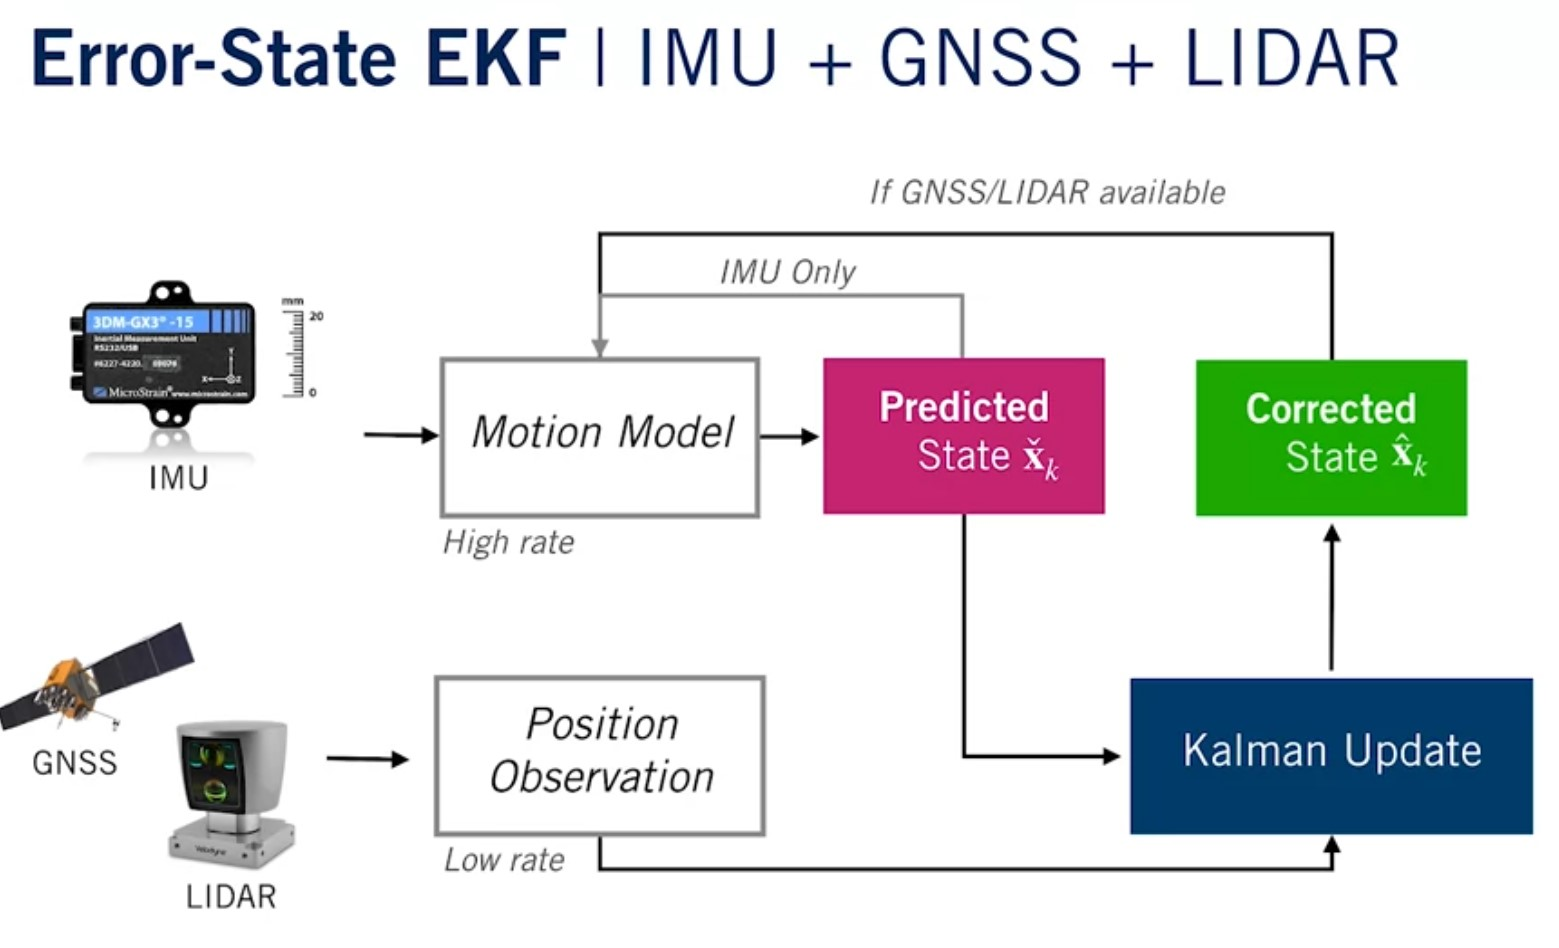
\includegraphics[scale=0.3]{eskf_pipeline.jpg}
\end{center}


\subsection{Физическая модель. Учебный пример}
\label{SubsectionPhysicalModelWarmup}

Допустим что у нас есть некоторая инерциальная система отсчета $C$ в которой мы
хотим определить координаты автомобиля $\pmb{r}\in\mathbb{R}^3$,
скорость $\pmb{v}\in\mathbb{R}^3$, ускорение $\pmb{a}\in\mathbb{R}^3$ и
ориентацию в виде кватерниона $\pmb{q}\in\mathbb{H}$,
Во время движения IMU будет измерять ускорение $\pmb{a}_m\in\mathbb{R}^3$ и
угловую скорость $\pmb{\omega}_m\in\mathbb{R}^3$ в своей системе координат
(назовем ее $A$). Для удобства начальной локализации мы будем следить
за вектором ускорения свободного падения $\pmb{g}$. Мы будем считать что
у IMU есть некоторая систематическая ошибка $\pmb{a}_b$ определения ускорения
и систематическая ошибка определения угловой скорости $\pmb{\omega}_b$. Скорости
изменения $\pmb{a}_b$ и $\pmb{\omega}_b$ будут случайными нормально
распределенными случайными величинами $\pmb{a}_w$, $\pmb{\omega}_w$ с нулевым
средним. Уравнения движения автомобиля в этом случае примут вид
\begin{equation}
    \begin{aligned}
        \frac{d \pmb{r}(t)}{d t}= & \pmb{v}(t)                                          \\
        \frac{d \pmb{v}(t)}{d t}= & \pmb{a}(t)                                          \\
        \frac{d \pmb{q}(t)}{d t}= & \frac{1}{2} \pmb{q}(t) \otimes q\{\pmb{\omega}(t)\}
    \end{aligned}
    \qquad \qquad
    \begin{aligned}
        \frac{d \pmb{a}_b(t)}{d t}=      & \pmb{a}_w(t)      \\
        \frac{d \pmb{\omega}_b(t)}{d t}= & \pmb{\omega}_w(t) \\
        \frac{d \pmb{g}(t)}{d t}=        & 0                 \\
    \end{aligned}
\end{equation}
При этом измерения IMU будут
\begin{equation}
    \begin{aligned}
        \pmb{a}_m(t)=      & R\{\pmb{q}(t)\}^T(\pmb{a}(t) - \pmb{g}(t)) + \pmb{a}_b(t) + \pmb{a}_n(t) \\
        \pmb{\omega}_m(t)= & \pmb{\omega}(t) + \pmb{\omega}_b(t) + \pmb{\omega}_n(t)
    \end{aligned}
\end{equation}
Следовательно,
\begin{equation}
    \begin{aligned}
        \frac{d \pmb{r}(t)}{d t}= & \pmb{v}(t)                                                                \\
        \frac{d \pmb{v}(t)}{d t}= & R\{\pmb{q}(t)\} (\pmb{a}_m(t) - \pmb{a}_b(t) - \pmb{a}_n(t)) + \pmb{g}(t) \\
        \frac{d \pmb{q}(t)}{d t}= & \frac{1}{2} \pmb{q}(t) \otimes q\{
        \pmb{\omega}_m(t) - \pmb{\omega}_b(t) - \pmb{\omega}_n(t)
        \}                                                                                                    \\
    \end{aligned}
    \qquad\qquad
    \begin{aligned}
        \frac{d \pmb{a}_b(t)}{d t}=      & \pmb{a}_w(t)      \\
        \frac{d \pmb{\omega}_b(t)}{d t}= & \pmb{\omega}_w(t) \\
        \frac{d \pmb{g}(t)}{d t}=        & 0                 \\
    \end{aligned}
\end{equation}

\subsubsection{Расширенный фильтр Калмана для локализации автомобиля}
\label{SubsubsectionExtendedKalmanFilterForLocalization}

Во время движения автомобиля мы будем получать измерения от лидара и навигатора.
Это будут либо позиция либо скорость либо ориентация. Теперь мы готовы описать
движение автомобиля как динамической системы:
\begin{equation}
    \pmb{x}(t)=\begin{bmatrix}
        \pmb{r}(t)   \\ \pmb{v}(t) \\ \pmb{q}(t) \\
        \pmb{a}_b(t) \\ \pmb{\omega}_b(t) \\ \pmb{g}(t)
    \end{bmatrix}
    \,
    \pmb{z}(t)=\begin{bmatrix}
        \pmb{r}(t) \\ \pmb{v}(t) \\ \pmb{q}(t)
    \end{bmatrix}
    \,
    u(t)=\begin{bmatrix}
        \pmb{a}_m(t) - \pmb{a}_n(t) \\
        \pmb{\omega}_m(t) - \pmb{\omega}_n(t)
    \end{bmatrix}
    \,
    \pmb{\mu}(t)=\begin{bmatrix}
        \pmb{a}_w(t) \\ \pmb{\omega}_w(t)
    \end{bmatrix}
    \,
    \pmb{\nu}(t)=\begin{bmatrix}
        \pmb{\nu}_r(t) \\ \pmb{\nu}_v(t) \\ \pmb{\nu}_q(t)
    \end{bmatrix}
\end{equation}
\begin{equation}
    f(t,\pmb{x},u,\pmb{\mu})=\begin{bmatrix}
        \pmb{v}                                                    \\
        R\{\pmb{q}\} (\pmb{a}_m - \pmb{a}_b - \pmb{a}_n) + \pmb{g} \\
        \frac{1}{2} \pmb{q} \otimes q\{
        \pmb{\omega}_m - \pmb{\omega}_b - \pmb{\omega}_n
        \}                                                         \\
        \pmb{a}_w(t)                                               \\
        \pmb{\omega}_w(t)                                          \\
        0                                                          \\
    \end{bmatrix}
    \qquad
    h(t,\pmb{x},\pmb{\nu})=\begin{bmatrix}
        \pmb{r} + \pmb{\nu}_r                           \\
        \pmb{v} + \pmb{\nu}_v                           \\
        \pmb{q} \otimes \operatorname{Exp}(\pmb{\nu}_q) \\
    \end{bmatrix}
\end{equation}
Видно, что получающаяся динамическая система нелинейная и оценивать ее динамику
лучше с помощью фильтра Калмана с состоянием ошибок.

\begin{remark} Строго говоря это динамическая система не определена корректно,
    так как между некоторыми координатами вектора сосотояний существует неявная
    зависимость, а именно $\Vert \pmb{q}\Vert=1$. Но мы, к сожалению, тут пожертвуем
    математической строгостью.
\end{remark}

\subsubsection{Расширенный фильтр Калмана с состоянием ошибок для локализации автомобиля}
\label{SubsubsectionErorStateKalmanFilterForLocalization}


Для построения фильтра Калмана с состоянием ошибок мы будем определим
номинальное состояние и состояние ошибок и реальное состояние следующим образом
\begin{equation}
    \bar{x}(t)=\begin{bmatrix}
        \bar{r}(t)   \\ \bar{v}(t) \\ \bar{q}(t) \\
        \bar{a}_b(t) \\ \bar{\omega}_b(t) \\ \bar{g}(t)
    \end{bmatrix}
    \qquad
    \delta \pmb{x}(t)=\begin{bmatrix}
        \delta \pmb{r}(t)   \\ \delta \pmb{v}(t) \\ \delta \pmb{\theta}(t) \\
        \delta \pmb{a}_b(t) \\ \delta \pmb{\omega}_b(t) \\ \delta \pmb{g}(t)
    \end{bmatrix}
\end{equation}
При этом реальное состояние будет связано с номинальным и состоянием ошибок следующим образом
\begin{equation}
    \pmb{x}(t)=\begin{bmatrix}
        \bar{r}(t) + \delta \pmb{r}(t)                              \\
        \bar{v}(t) + \delta \pmb{v}(t)                              \\
        \bar{q}(t)\otimes\operatorname{Exp}(\delta \pmb{\theta}(t)) \\
        \bar{a}_b(t) + \delta \pmb{a}_b(t)                          \\
        \bar{\omega}_b(t) + \delta \pmb{\omega}_b(t)                \\
        \bar{g}(t) + \delta \pmb{g}(t)
    \end{bmatrix}
\end{equation}
Динамика номинального состояния описывается уравнениями не учитывающими шум и ошибки.
\begin{equation}
    \begin{aligned}
        \frac{d \bar{r}(t)}{d t}= & \bar{v}(t)                                                 \\
        \frac{d \bar{v}(t)}{d t}= & R\{\bar{q}(t)\} (\pmb{a}_m(t) - \bar{a}_b(t)) + \bar{g}(t) \\
        \frac{d \bar{q}(t)}{d t}= & \frac{1}{2} \bar{q}(t) \otimes q\{
        \pmb{\omega}_m(t) - \bar{\omega}_b(t)
        \}                                                                                     \\
    \end{aligned}
    \qquad\qquad
    \begin{aligned}
        \frac{d \bar{a}_b(t)}{d t}=      & 0 \\
        \frac{d \bar{\omega}_b(t)}{d t}= & 0 \\
        \frac{d \bar{g}(t)}{d t}=        & 0 \\
    \end{aligned}
\end{equation}
Динамика состояния ошибок выводится из уравнения для реального состояния,
уравнений для номинального состояния и связи между реальным, номинальным и состоянием ошибок.
Начнем с простых уравнений
\begin{equation}
    \begin{aligned}
        \frac{d \delta\pmb{r}(t)}{d t}
        = & \frac{d \pmb{r}(t)}{dt} - \frac{d\bar{r}(t)}{d t}
        =\pmb{v}(t)-\bar{v}(t)
        =\delta\pmb{v}(t)                                                   \\
        \frac{d \delta\pmb{a}_b(t)}{d t}
        = & \frac{d \pmb{a}_b(t)}{dt} - \frac{d\bar{a}_b(t)}{d t}
        =\pmb{a}_w(t)-0
        =\pmb{a}_w(t)                                                       \\
        \frac{d \delta\pmb{\omega}_b(t)}{d t}
        = & \frac{d \pmb{\omega}_b(t)}{dt} - \frac{d\bar{\omega}_b(t)}{d t}
        =\pmb{\omega}_w(t) - 0
        =\pmb{\omega}_w(t)                                                  \\
        \frac{d \delta\pmb{g}(t)}{d t}
        = & \frac{d \pmb{g}(t)}{dt} - \frac{d\bar{g}(t)}{d t}
        =0                                                                  \\
    \end{aligned}
\end{equation}
Выведем уравенение для ошибки скорости. Обозначим
\begin{equation}
    \pmb{a}_{mb}(t)=\pmb{a}_m(t)-\bar{a}_b(t)  \qquad
    \delta \pmb{a}_{mb}(t)=-\delta \pmb{a}_b(t)-\pmb{a}_n(t)  \qquad
    \pmb{R}(t)=R\{\pmb{q}(t)\} \quad
    \bar{R}(t)=R\{\bar{q}(t)\}
\end{equation}
Тогда
\begin{equation}
    \frac{d \pmb{v}(t)}{d t}=\pmb{R}(t) (\pmb{a}_{mb}(t)+\delta\pmb{a}_{mb}(t)) + \pmb{g}(t)\\
    \qquad
    \frac{d \bar{v}(t)}{d t}=\bar{R}(t) \pmb{a}_{mb}(t) + \bar{g}(t)\\
\end{equation}
Учитывая, что
\begin{equation}
    \pmb{R}(t)=\bar{R}(t)(I+[\delta\pmb{\theta}(t)]_\times+o(\delta\pmb{\theta}(t)))
\end{equation}
получим
\begin{equation}
    \begin{aligned}
        \frac{d \delta \pmb{v}(t)}{dt}
        = &
        \frac{d \pmb{v}(t)}{dt} - \frac{ d\bar{v}(t)}{dt}                                                          \\
        = &
        (\pmb{R}(t) (\pmb{a}_{mb}(t)+\delta\pmb{a}_{mb}(t)) + \pmb{g}(t))                                          \\
          &
        - (\bar{R}(t) \pmb{a}_{mb}(t) + \bar{g}(t))                                                                \\
        = &
        \bar{R}(t)(I+[\delta\pmb{\theta}(t)]_\times+o(\delta\pmb{\theta})) (\pmb{a}_{mb}(t)+\delta\pmb{a}_{mb}(t)) \\
          &
        - \bar{R}(t) \pmb{a}_{mb}(t) + \pmb{g}(t) - \bar{g}(t)                                                     \\
        = &
        \bar{R}(t) (\pmb{a}_{mb}(t)+\delta\pmb{a}_{mb}(t))
        + \bar{R}(t)[\delta\pmb{\theta}(t)]_\times (\pmb{a}_{mb}(t)+\delta\pmb{a}_{mb}(t))
        + o(\delta\pmb{\theta}(t))                                                                                 \\
          &
        - \bar{R}(t) \pmb{a}_{mb}(t) + \delta\pmb{g}(t)                                                            \\
        = &
        \bar{R}(t) \delta\pmb{a}_{mb}(t)
        + \bar{R}(t)[\delta\pmb{\theta}(t)]_\times (\pmb{a}_{mb}(t)                                                \\
          &
        +\delta\pmb{a}_{mb}(t))
        + \delta\pmb{g}(t)
        + o(\delta\pmb{\theta}(t))                                                                                 \\
        = &
        \bar{R}(t) \delta\pmb{a}_{mb}(t)
        + \bar{R}(t)[\delta\pmb{\theta}(t)]_\times \pmb{a}_{mb}(t)                                                 \\
          &
        + \bar{R}(t)[\delta\pmb{\theta}(t)]_\times \delta\pmb{a}_{mb}(t)
        + \delta\pmb{g}(t)
        + o(\delta\pmb{\theta}(t))                                                                                 \\
        = &
        - \bar{R}(t) \delta\pmb{a}_{b}(t)
        - \bar{R}(t) \pmb{a}_{n}(t)
        - \bar{R}(t)[\pmb{a}_{mb}(t)]_\times \delta\pmb{\theta}(t)
        - \bar{R}(t)[\delta\pmb{\theta}(t)]_\times \delta\pmb{a}_{b}(t)                                            \\
          &
        - \bar{R}(t)[\delta\pmb{\theta}(t)]_\times \pmb{a}_{n}(t)
        + \delta\pmb{g}(t)
        + o(\delta\pmb{\theta}(t))                                                                                 \\
        = &
        - \bar{R}(t) \delta\pmb{a}_{b}(t)
        - \bar{R}(t)[\pmb{a}_{m}(t) - \bar{a}_b(t)]_\times \delta\pmb{\theta}(t)
        - o(\delta\pmb{\theta}(t))                                                                                 \\
          &
        - \bar{R}(t) \pmb{a}_{n}(t)
        - \bar{R}(t)[\delta\pmb{\theta}(t)]_\times \pmb{a}_{n}(t)
        + \delta\pmb{g}(t)
        + o(\delta\pmb{\theta}(t))                                                                                 \\
        = &
        - \bar{R}(t) \delta\pmb{a}_{b}(t)
        - \bar{R}(t)[\pmb{a}_{m}(t) - \bar{a}_b(t)]_\times \delta\pmb{\theta}(t)                                   \\
          &
        - \bar{R}(t)(I+[\delta\pmb{\theta}(t)]_\times) \pmb{a}_{n}(t)
        + \delta\pmb{g}(t)
        + o(\delta\pmb{\theta}(t))                                                                                 \\
    \end{aligned}
\end{equation}
Мы не будем выводить явные форумулы для членов второго порядка малости, поэтому
\begin{equation}
    \begin{aligned}
        \frac{d \delta \pmb{v}(t)}{dt}
        = & -\bar{R}(t)\delta\pmb{a}_b(t)
        -\bar{R}(t)[\pmb{a}_m(t) - \bar{a}_b(t)]_\times \delta\pmb{\theta}(t)      \\
          & + o(\Vert\delta\pmb{\theta}(t)\Vert)
        + o(\Vert\delta\pmb{\theta}(t)\Vert)
        - \bar{R}(t)\pmb{a}_n(t)
        - \bar{R}(t)[\delta\pmb{\theta}(t)]_\times\pmb{a}_n(t)
        + \delta \pmb{g}(t)                                                        \\
        = & - \bar{R}(t)[\pmb{a}_m(t) - \bar{a}_b(t)]_\times \delta\pmb{\theta}(t)
        - \bar{R}(t)\delta\pmb{a}_b(t)                                             \\
          & + \delta \pmb{g}(t)
        - \bar{R}(t)(I+[\delta\pmb{\theta}(t)]_\times)\pmb{a}_n(t)
        + o(\delta\pmb{\theta}(t))                                                 \\
    \end{aligned}
\end{equation}
Теперь выведем уравнение для ошибки угловой скорости. Обозначим
\begin{equation}
    \pmb{\omega}_{mb}(t)=\pmb{\omega}_m(t) - \bar{\omega}_b(t) \qquad
    \delta\pmb{\omega}_{mb}(t)=-\delta\pmb{\omega}_b(t) - \pmb{\omega}_n(t) \qquad
\end{equation}
Тогда
\begin{equation}
    \frac{d \pmb{q}(t)}{dt}=\frac{1}{2}\pmb{q}(t)\otimes q\{\pmb{\omega}_{mb}(t)\}
    \qquad
    \frac{d \bar{q}(t)}{dt}=\frac{1}{2}\bar{q}(t)\otimes q\{\pmb{\omega}_{mb}(t)+\delta \pmb{\omega}_{mb}(t)\}
    \qquad
    \pmb{q}(t)=\bar{q}(t)\otimes \delta\pmb{q}(t)
\end{equation}
Находим
\begin{equation}
    \begin{aligned}
        \frac{d \pmb{q}(t)}{d t}
         & =\frac{d}{d t}(\bar{q}(t)\otimes \delta\pmb{q}(t))                                                          \\
        \frac{1}{2}\pmb{q}(t)\otimes q\{\pmb{\omega}_{mb}(t)\}
         & =\frac{d\bar{q}(t)}{d t}\otimes \delta\pmb{q}(t)
        +\bar{q}(t)\otimes \frac{d\delta\pmb{q}(t)}{d t}                                                               \\
        \frac{1}{2}\pmb{q}(t)\otimes q\{\pmb{\omega}_{mb}(t)\}
         & =\frac{1}{2}\bar{q}(t)\otimes q\{\pmb{\omega}_{mb}(t)+\delta \pmb{\omega}_{mb}(t)\}\otimes \delta\pmb{q}(t)
        +\bar{q}(t)\otimes \frac{d\delta\pmb{q}(t)}{d t}                                                               \\
        \frac{1}{2}\bar{q}(t)\otimes \delta\pmb{q}(t) \otimes q\{\pmb{\omega}_{mb}(t)\}
         & =\frac{1}{2}\bar{q}(t)\otimes q\{\pmb{\omega}_{mb}(t)+\delta \pmb{\omega}_{mb}(t)\}\otimes \delta\pmb{q}(t)
        +\bar{q}(t)\otimes \frac{d\delta\pmb{q}(t)}{d t}                                                               \\
        \frac{1}{2}\delta\pmb{q}(t) \otimes q\{\pmb{\omega}_{mb}(t)\}
         & =\frac{1}{2}q\{\pmb{\omega}_{mb}(t)+\delta \pmb{\omega}_{mb}(t)\}\otimes \delta\pmb{q}(t)
        +\frac{d\delta\pmb{q}(t)}{d t}                                                                                 \\
        \frac{d\delta\pmb{q}(t)}{d t}
         & = \frac{1}{2}\left(\delta\pmb{q}(t) \otimes q\{\pmb{\omega}_{mb}(t)\}-
        q\{\pmb{\omega}_{mb}(t)+\delta \pmb{\omega}_{mb}(t)\}\otimes \delta\pmb{q}(t) \right)                          \\
    \end{aligned}
\end{equation}
Домножая на $\bar{q}^{-1}$ мы получим
\begin{equation}
    \begin{aligned}
        \frac{d\delta\pmb{q}(t)}{d t}
         & = \frac{1}{2}\left(\delta\pmb{q}(t) \otimes q\{\pmb{\omega}_{mb}(t)\}-
        q\{\pmb{\omega}_{mb}(t)+\delta \pmb{\omega}_{mb}(t)\}\otimes \delta\pmb{q}(t)\right) \\
         & = \frac{1}{2}([q\{\pmb{\omega}_{mb}(t)\}]_R \delta\pmb{q}(t) -
        [q\{\pmb{\omega}_{mb}(t)+\delta \pmb{\omega}_{mb}(t)\}]_L) \delta\pmb{q}(t)          \\
         & = \frac{1}{2}\left(
        \left[
            \begin{bmatrix}
                0 \\ \pmb{\omega}_{mb}(t)
            \end{bmatrix}
            \right]_R -
        \left[
            \begin{bmatrix}
                0 \\ \pmb{\omega}_{mb}(t)+\delta \pmb{\omega}_{mb}(t)
            \end{bmatrix}
            \right]_L
        \right) \delta\pmb{q}(t)                                                             \\
         & = \frac{1}{2}\left(
        \begin{bmatrix}
                0                    & -\pmb{\omega}_{mb}(t)^T        \\
                \pmb{\omega}_{mb}(t) & -[\pmb{\omega}_{mb}(t)]_\times \\
            \end{bmatrix}
        -
        \begin{bmatrix}
                0                                                & -(\pmb{\omega}_{mb}(t)+\delta \pmb{\omega}_{m(t)b})^T     \\
                \pmb{\omega}_{mb}(t)+\delta \pmb{\omega}_{mb}(t) & [\pmb{\omega}_{mb}(t)+\delta \pmb{\omega}_{mb}(t)]_\times \\
            \end{bmatrix}
        \right) \delta\pmb{q}(t)                                                             \\
         & =
        \frac{1}{2}\begin{bmatrix}
            0                          & -\delta\pmb{\omega}_{mb}(t)^T                              \\
            \delta\pmb{\omega}_{mb}(t) & -[2\pmb{\omega}_{mb}(t)+\delta\pmb{\omega}_{mb}(t)]_\times \\
        \end{bmatrix}
        \delta\pmb{q}(t)                                                                     \\
    \end{aligned}
\end{equation}
Поскольку $\delta\pmb{q}(t)=\operatorname{Exp}(\delta\pmb{\theta}(t))=[1, \delta\pmb{\theta}(t)/2]^T+o(\delta\pmb{\theta})$,
мы получаем равенства
\begin{equation}
    \begin{aligned}
        \frac{d}{d t}\begin{bmatrix}1 \\ \delta\pmb{\theta}(t)/2\end{bmatrix}+o(\delta\pmb{\theta})
         & =
        \frac{1}{2}\begin{bmatrix}
            0                          & -\delta\pmb{\omega}_{mb}(t)^T                              \\
            \delta\pmb{\omega}_{mb}(t) & -[2\pmb{\omega}_{mb}(t)+\delta\pmb{\omega}_{mb}(t)]_\times \\
        \end{bmatrix}
        \begin{bmatrix}1 \\ \delta\pmb{\theta}(t)/2\end{bmatrix} + o(\delta\pmb{\theta}(t)) \\
        \frac{d}{d t}\begin{bmatrix}1 \\ \delta\pmb{\theta}(t)\end{bmatrix}
         & =
        \begin{bmatrix}
            -\frac{1}{2}\delta\pmb{\omega}_{mb}(t)^T \delta\pmb{\theta}(t)                                                        \\
            \delta\pmb{\omega}_{mb}(t)-\frac{1}{2}[2\pmb{\omega}_{mb}(t)+\delta\pmb{\omega}_{mb}(t)]_\times \delta\pmb{\theta}(t) \\
        \end{bmatrix}
        + o(\delta\pmb{\theta}(t))                            \\
    \end{aligned}
\end{equation}
В частности
\begin{equation}
    \begin{aligned}
        \frac{d\delta\pmb{\theta}(t)}{dt}
         & =\delta\pmb{\omega}_{mb}(t)
        - [\pmb{\omega}_{mb}(t)]_\times\delta\pmb{\theta}(t)
        - \frac{1}{2}[\delta\pmb{\omega}_{mb}(t)]_\times \delta\pmb{\theta}(t)
        + o(\delta\pmb{\theta}(t))                                                 \\
         & = - \delta\pmb{\omega}_{b}(t) - \pmb{\omega}_n(t)
        - [\pmb{\omega}_{m}(t)-\bar{\omega}_b(t)]_\times\delta\pmb{\theta}(t)
        + o(\delta\pmb{\theta}(t))
        + o(\delta\pmb{\theta}(t))                                                 \\
         & = - [\pmb{\omega}_{m}(t)-\bar{\omega}_b(t)]_\times\delta\pmb{\theta}(t)
        - \delta\pmb{\omega}_{b}(t) - \pmb{\omega}_n(t)
        + o(\delta\pmb{\theta}(t))
    \end{aligned}
\end{equation}

Таким образом
\begin{equation}
    \begin{aligned}
        \frac{d \delta\pmb{r}(t)}{d t}=        & \delta\pmb{v}(t)                                                           \\
        \frac{d \delta\pmb{v}(t)}{d t}
        =                                      & -R\{\bar{q}(t)\} [\pmb{a}_m(t) - \bar{a}_b(t)]_\times\delta\pmb{\theta}(t)
        - R\{\bar{q}(t)\} \delta\pmb{a}_b(t)
        + \delta\pmb{g}(t)                                                                                                  \\
                                               & - R\{\bar{q}(t)\}(I+[\delta\pmb{\theta}(t)]_\times) \pmb{a}_n(t)
        + o(\delta\pmb{\theta}(t))                                                                                          \\
        \frac{d \delta\pmb{\theta}(t)}{d t}=   & -[\pmb{\omega}_m(t) - \bar{\omega}_b(t)]_\times \delta \pmb{\theta}(t)
        - \delta \pmb{\omega}_b(t)
        - \pmb{\omega}_n(t) + o(\delta\pmb{\theta}(t))                                                                      \\
        \frac{d \delta\pmb{a}_b(t)}{d t}=      & \pmb{a}_w(t)                                                               \\
        \frac{d \delta\pmb{\omega}_b(t)}{d t}= & \pmb{\omega}_w(t)                                                          \\
        \frac{d \delta\pmb{g}(t)}{d t}=        & 0                                                                          \\
    \end{aligned}
\end{equation}

Дискретизация уравнений номинального сосотояния будет
\begin{equation}
    \begin{aligned}
        \bar{r}_k=          & \bar{r}_{k-1} + \bar{v}_{k-1} \Delta t
        + (R\{\bar{q}_{k-1}\} (\pmb{a}_{m,k} - \bar{a}_{b,k-1})
        + \bar{g}_{k-1}) \frac{\Delta t^2}{2}                                                                                 \\
        \bar{v}_k=          & \bar{v}_{k-1} + (R\{\bar{q}_{k-1}\} (\pmb{a}_{m,k} - \bar{a}_{b,k-1}) + \bar{g}_{k-1}) \Delta t \\
        \bar{q}_k=          & \bar{q}_{k-1} \otimes q\{(\pmb{\omega}_{m,k} - \bar{\omega}_{b,k-1})\Delta t\}                  \\
        \bar{a}_{b,k}=      & \bar{a}_{b,k-1}                                                                                 \\
        \bar{\omega}_{b,k}= & \bar{\omega}_{b,k-1}                                                                            \\
        \bar{g}_{k}=        & \bar{g}_{k-1}                                                                                   \\
    \end{aligned}
\end{equation}
Дискретизация уравнений сосотояния ошибки имеет вид
\begin{equation}
    \begin{aligned}
        \delta\pmb{r}_k=          & \delta\pmb{r}_{k-1} + \delta\pmb{v}_{k-1} \Delta t                                          \\
        \delta\pmb{v}_k=          & \delta \pmb{v}_{k-1}
        - R\{\bar{q}_{k-1}\} [\pmb{a}_{m, k} - \bar{a}_{b, k-1}]_\times\delta\pmb{\theta}_{k-1} \Delta t                        \\
                                  & - R\{\bar{q}_{k-1}\} \delta\pmb{a}_{b,k-1} \Delta t
        + \delta\pmb{g}_{k-1} \Delta t
        - R\{\bar{q}_{k-1}\}(I+[\delta\pmb{\theta}_{k-1}]_\times) \pmb{a}_{n,k} \Delta t                                        \\
        \delta\pmb{\theta}_k=     & R\{-[\pmb{\omega}_{m,k} - \bar{\omega}_{b,k-1}]_\times \Delta t\} \delta \pmb{\theta}_{k-1}
        - \delta \pmb{\omega}_{b,k-1} \Delta t
        - \pmb{\omega}_{n,k} \Delta t                                                                                           \\
        \delta\pmb{a}_{b,k}=      & \delta\pmb{a}_{b,k-1} + \pmb{a}_{w, k} \Delta t                                             \\
        \delta\pmb{\omega}_{b,k}= & \delta\pmb{\omega}_{b,k-1} + \pmb{\omega}_{w,k} \Delta t                                    \\
        \delta\pmb{g}_k=          & \delta\pmb{g}_{k-1}                                                                         \\
    \end{aligned}
\end{equation}

Полученным уравнениям соответствует динамическая система
{\small
\begin{equation}
    \bar{x}_{k}=\begin{bmatrix}
        \bar{r}_{k}   \\ \bar{v}_{k} \\ \bar{q}_{k} \\
        \bar{a}_{b,k} \\ \bar{\omega}_{b,k} \\ \bar{g}_{k}
    \end{bmatrix}
    \quad
    \delta \pmb{x}_{k}=\begin{bmatrix}
        \delta \pmb{r}_{k}   \\ \delta \pmb{v}_{k} \\ \delta \pmb{\theta}_{k} \\
        \delta \pmb{a}_{b,k} \\ \delta \pmb{\omega}_{b,k} \\ \delta \pmb{g}_{k}
    \end{bmatrix}
    \quad
    \pmb{z}_{k}=\begin{bmatrix}
        \pmb{r}_{k} \\ \pmb{v}_{k} \\ \pmb{q}_{k}
    \end{bmatrix}
    \quad
    u_{k}=\begin{bmatrix}
        \pmb{a}_{m,k} \\
        \pmb{\omega}_{m,k}
    \end{bmatrix}
    \quad
    \pmb{\mu}_{k}=\begin{bmatrix}
        \pmb{a}_{n,k} \\ \pmb{\omega}_{n,k} \\
        \pmb{a}_{w,k} \\ \pmb{\omega}_{w,k}
    \end{bmatrix}
    \quad
    \pmb{\nu}_{k}=\begin{bmatrix}
        \pmb{\nu}_{r,k} \\ \pmb{\nu}_{v,k} \\ \pmb{\nu}_{q,k}
    \end{bmatrix}
\end{equation}
\begin{equation}
    \begin{aligned}
        \bar{f}_k(\bar{x},u)=\begin{bmatrix}
            \bar{r} + \bar{v} \Delta t
            + (R\{\bar{q}\} (\pmb{a}_{m} - \bar{a}_{b})
            + \bar{g}) \frac{\Delta t^2}{2}                                    \\
            \bar{v} + R\{\bar{q}\} (\pmb{a}_{m} - \bar{a}_{b}) \Delta t        \\
            \bar{q} \otimes q\{(\pmb{\omega}_{m} - \bar{\omega}_{b})\Delta t\} \\
            \bar{a}_{b}                                                        \\
            \bar{\omega}_{b}                                                   \\
            \bar{g}                                                            \\
        \end{bmatrix}
    \end{aligned}
    \quad
    \begin{aligned}
        h_k(\bar{x}, \delta\pmb{x}, \nu) & =\begin{bmatrix}
            \bar{r} + \delta\pmb{r}+\pmb{\nu}_{r}                                                            \\
            \bar{v} + \delta\pmb{v}+\pmb{\nu}_{v}                                                            \\
            \bar{q} \otimes \operatorname{Exp}(\delta\pmb{\theta}) \otimes \operatorname{Exp}(\pmb{\nu}_{q}) \\
        \end{bmatrix}
    \end{aligned}
\end{equation}
\begin{equation}
    \begin{aligned}
        \delta f_k(\bar{x},\delta \pmb{x}, u, \pmb{\mu})=\begin{bmatrix}
            \delta\pmb{r} + \delta\pmb{v} \Delta t                             \\
            \delta \pmb{v}
            - R\{\bar{q}\} [\pmb{a}_{m} - \bar{a}_{b}]_\times\delta\pmb{\theta} \Delta t
            - R\{\bar{q}\} \delta\pmb{a}_{b} \Delta t
            + \delta\pmb{g} \Delta t
            - R\{\bar{q}\}(I+[\delta\pmb{\theta}]_\times) \pmb{a}_{n} \Delta t \\
            R\{-[\pmb{\omega}_{m} - \bar{\omega}_{b}]_\times \Delta t\} \delta \pmb{\theta}
            - \delta \pmb{\omega}_{b} \Delta t
            - \pmb{\omega}_{n} \Delta t                                        \\
            \delta\pmb{a}_{b} + \pmb{a}_{w} \Delta t                           \\
            \delta\pmb{\omega}_{b} + \pmb{\omega}_{w} \Delta t                 \\
            \delta\pmb{g}                                                      \\
        \end{bmatrix}
    \end{aligned}
\end{equation}
\begin{equation}
    s_k(\bar{x}, \delta\pmb{x})=\begin{bmatrix}
        \bar{r} + \delta\pmb{r}                                \\
        \bar{v} + \delta\pmb{v}                                \\
        \bar{q} \otimes \operatorname{Exp}(\delta\pmb{\theta}) \\
        \bar{a}_b + \delta\pmb{a}_b                            \\
        \bar{\omega}_b + \delta\pmb{\omega}_b                  \\
        \bar{g} + \delta\pmb{g}                                \\
    \end{bmatrix}
\end{equation}
}
Функция $g_k$ определяемая из уравнения  $s_k(x_{k|k}, g_k(\delta x))=s_k(\bar{x}_{k}, \delta x)$
не имеет аналитической формулы, но есть преближенная:
\begin{equation}
    g_k(\delta\pmb{x})=\begin{bmatrix}
        \delta\pmb{r} - \delta r_{k|k}                                                                                     \\
        \delta\pmb{v} - \delta v_{k|k}                                                                                     \\
        \left(I - \frac{1}{2}[\delta \theta_{k|k}]_\times \right) \delta \theta - \delta \theta_{k|k} + o(\delta \theta^2) \\
        \delta\pmb{a}_b - \delta a_{b,k|k}                                                                                 \\
        \delta\pmb{\omega}_b - \delta \omega_{b,k|k}                                                                       \\
        \delta\pmb{g} - \delta g_{k|k}                                                                                     \\
    \end{bmatrix}
\end{equation}

Чтобы применить алгоритм параграфа \ref{SubsectionErrorStateKalmanFilter} достаточно найти
несколько матриц
\begin{equation}
    \begin{aligned}
        F=\frac{\partial \delta f_k}{\partial \delta x}(\bar{x}, \delta\pmb{x}, u, 0)
         & =\begin{bmatrix}
            I & I\Delta t & 0                                                       & 0                     & 0          & 0          \\
            0 & I         & -R\{\bar{q}\}\Delta t[\pmb{a}_m-\bar{a}_b]_\times       & -R\{\bar{q}\}\Delta t & 0          & I \Delta t \\
            0 & 0         & R\{-[\pmb{\omega}_m - \bar{\omega}_b]_\times \Delta t\} & 0                     & -I\Delta t & 0          \\
            0 & 0         & 0                                                       & I                     & 0          & 0          \\
            0 & 0         & 0                                                       & 0                     & I          & 0          \\
            0 & 0         & 0                                                       & 0                     & 0          & I          \\
        \end{bmatrix} \\
        L=\frac{\partial \delta f_k}{\partial \delta \mu}(\bar{x}, \delta\pmb{x}, u, 0)
         & =\begin{bmatrix}
            0                                                    & 0          & 0          & 0          \\
            -R\{\bar{q}\}(I+[\delta\pmb{\theta}]_\times)\Delta t & 0          & 0          & 0          \\
            0                                                    & I \Delta t & 0          & 0          \\
            0                                                    & 0          & I \Delta t & 0          \\
            0                                                    & 0          & 0          & I \Delta t \\
            0                                                    & 0          & 0          & 0          \\
        \end{bmatrix} \\
        H=\frac{\partial h_k}{\partial \delta x}(x,\delta\pmb{x}, 0)
         & =\begin{bmatrix}
            I & 0 & 0                                      & 0 & 0 & 0 \\
            0 & I & 0                                      & 0 & 0 & 0 \\
            0 & 0 & R\{\bar{q}\}^T J_r(\delta\pmb{\theta}) & 0 & 0 & 0 \\
        \end{bmatrix} \\
        M=\frac{\partial h_k}{\partial \nu}(x,\delta\pmb{x}, 0)
         & =\begin{bmatrix}
            I & 0 & 0 \\
            0 & I & 0 \\
            0 & 0 & I \\
        \end{bmatrix} \\
        G=\frac{\partial g_k}{\partial \delta x}(\delta x_{k|k})
         & =\begin{bmatrix}
            I & 0 & 0                                          & 0 & 0 & 0 \\
            0 & I & 0                                          & 0 & 0 & 0 \\
            0 & 0 & I - \frac{1}{2}[\delta\theta_{k|k}]_\times & 0 & 0 & 0 \\
            0 & 0 & 0                                          & I & 0 & 0 \\
            0 & 0 & 0                                          & 0 & I & 0 \\
            0 & 0 & 0                                          & 0 & 0 & I \\
        \end{bmatrix} \\
    \end{aligned}
\end{equation}


\section{Справочные материалы и обозначения}
\label{SectionAppendix}

\subsection{Кватернионы}
\label{SubsectionQuaternions}

Кватернион $q$ это пара из числа и вектора $[w, \vv{v}]^T$. Множество всех
кватеринионов будем обозначать $\mathbb{H}$. Пусть нам заданы два
кватерниона $q_1=[w_1,\vv{v}_1]^T$ и $q_2=[w_2,\vv{v}_2]^T$ и
числа $t_1,t_2\in\mathbb{R}$, тогда определим линейные операции над
кватеринионами
\begin{equation}
    t_1 q_1+ t_2 q_2=\begin{bmatrix}
        t_1 w_1 + t_2 w_2 \\ t_1 \vv{v}_1 + t_2 \vv{v}_2
    \end{bmatrix}
\end{equation}
Умножение кватернионов определяется по формуле
\begin{equation}
    q_1\otimes q_2
    =\begin{bmatrix} w_1 \\ \vv{v}_1\end{bmatrix}
    \otimes
    \begin{bmatrix} w_2 \\ \vv{v}_2\end{bmatrix}
    =\begin{bmatrix}
        w_1 w_2 - \vv{v}_1^T\vv{v}_2 \\
        w_1 \vv{v}_2 + w_2 \vv{v}_1 + \vv{v}_1\times \vv{v}_2
    \end{bmatrix},
\end{equation}
Умножение кватернионов некоммутативно (то есть зависит от порядка множителей).
Для любых кватернионов $q_1, q_2, q_3\in\mathbb{H}$ выполнены законы
ассоциативности и дистрибутивности
\begin{equation}
    (q_1+q_2)\otimes q_3=q_1\otimes q_3 + q_2\otimes q_3
    \quad
    q_3\otimes (q_1+q_2)=q_3\otimes q_1 + q_3\otimes q_2
    \quad
    (q_1\otimes q_2)\otimes q_3=q_1\otimes(q_2\otimes q_3)
\end{equation}

Кватернои вида $e=[1, 0]^T$ называется единичным и обладает тем свойством, что
$e \otimes q=q \otimes e=q$ для любого кватерниона $q\in\mathbb{H}$.

Каждый из множителей в формуле произведения кватернионов можно расматривать
как линейный оператор над четырехмерными векторами
\begin{equation}
    [q_1]_Lq_2=q_1\otimes q_2=[q_2]_Rq_1
\end{equation}
Откуда можно вывести, что
\begin{equation}
    [q]_L=w I+\begin{bmatrix}
        0 & -\vv{v}^T \\ \vv{v} & [\vv{v}]_\times
    \end{bmatrix}
    \qquad
    [q]_R=w I+\begin{bmatrix}
        0 & -\vv{v}^T \\ \vv{v} & -[\vv{v}]_\times
    \end{bmatrix}
\end{equation}
где
\begin{equation}
    [\vv{v}]_\times=\begin{bmatrix}
        0    & -v_3 & v_2  \\
        v_3  & 0    & -v_1 \\
        -v_2 & v_1  & 0    \\
    \end{bmatrix}
\end{equation}

Норма кватерниона определяется по формуле
\begin{equation}
    \Vert q\Vert=\sqrt{w^2+\vv{v}^T\vv{v}}
\end{equation}

Для заданного кватерниона его опряженный кватернион определеятся по формуле
\begin{equation}
    q^*=[w, -\vv{v}]^T
\end{equation}

Для любого ненулевого кватерниона $q\in\mathbb{H}$ существует обратный кватернион
$q^{-1}\in\mathbb{H}$ такой, что $q \otimes q^{-1} = q \otimes q^{-1}=e$. Более
того
\begin{equation}
    q^{-1}=\frac{q^*}{\Vert q\Vert^2}
\end{equation}

Действительная и мнимая часть кватерниона $q=[w,\vv{v}]$ определяется формулами
\begin{equation}
    \Re q= w \qquad \Im q=\vv{v}
\end{equation}
Легко проверить, что
\begin{equation}
    \Vert q\Vert=\sqrt{\Re(q\otimes q^*)}
    \qquad
    \Vert p \otimes q\Vert=\Vert p\Vert \Vert q\Vert
\end{equation}


Кватернионы у которых первая компонента равна 0 называются чистыми. Для заданного
числа $w\in\mathbb{R}$ и вектора $\vv{v}\in\mathbb{R}^3$ введем обозначения
\begin{equation}
    q\{w\}=\begin{bmatrix}
        w \\ 0
    \end{bmatrix}
    \qquad
    q\{\vv{v}\}=\begin{bmatrix}
        0 \\ \vv{v}
    \end{bmatrix}
\end{equation}
Множество чистых кватернионов мы будем обозначать через $\mathbb{H}_p$.

Кватернионы нормы 1 называются единичными. Если $q$ -- единичный кватернион, то
\begin{equation}
    q=\begin{bmatrix}
        \cos t \\ \vv{u} \sin t
    \end{bmatrix}
    =\cos t \cdot e + \sin t \cdot q\{\vv{u}\}
\end{equation}
где $\vv{u}$ -- вектор единичной длины и $t\in\mathbb{R}$. Для такого кватерниона
обратный находится очень просто
\begin{equation}
    q^{-1}=\begin{bmatrix}
        \cos \theta \\ -\vv{u} \sin\theta
    \end{bmatrix}
\end{equation}
Множество единичных кватернионов мы будем обозначать $S^3$.


Для кватернионов можно определить аналоги стандартных функций.
Пусть $q=[w,\vv{v}]^T$ -- некоторый кватернион, тогда положим по определению
\begin{equation}
    \exp:\mathbb{H}\to\mathbb{H}:q\mapsto e^w\begin{bmatrix}
        \cos \Vert \vv{v}\Vert \\
        \frac{\vv{v}}{\Vert\vv{v}\Vert}\sin\Vert\vv{v}\Vert
    \end{bmatrix}
    \qquad
    \log:\mathbb{H}\to\mathbb{H}:q\mapsto \begin{bmatrix}
        \log \sqrt{w^2+\vv{v}^T\vv{v}} \\
        \frac{\vv{v}}{\Vert\vv{v}\Vert}\arctan\frac{\Vert\vv{v}\Vert}{w}
    \end{bmatrix}
\end{equation}
Можно показать, что эти функции взаимно обратные друг к другу.

Аналогично можно определить экспоненту от вектора и логарифм от единичного кватерниона
\begin{equation}
    \begin{aligned}
        \exp: & \mathbb{R}^3\to S^3:
        \vv{v}\mapsto
        \begin{bmatrix}
            \cos \Vert \vv{v}\Vert \\
            \frac{\vv{v}}{\Vert \vv{v}\Vert}\sin\Vert \vv{v}\Vert
        \end{bmatrix}
        \\
        \log: & S^3\to\mathbb{H}_p:q\mapsto\begin{bmatrix}
            0 \\
            \frac{\vv{v}}{\Vert\vv{v}\Vert}\arctan\frac{\Vert\vv{v}\Vert}{w}
        \end{bmatrix}
    \end{aligned}
\end{equation}
Легко проверить, что
\begin{equation}
    \exp(\vv{v})=\exp(q\{\vv{v}\})
    \qquad
    \exp(q)^{-1}=\exp(q^*)
    \qquad
    \exp(\vv{v})^{-1}=\exp(-\vv{v})
\end{equation}
Нам будет полезен еще один вид экспоненты и логарифма
\begin{equation}
    \operatorname{Exp}:\mathbb{R}^3\to S^3:
    \vv{v}\mapsto\exp\left(\frac{1}{2}\vv{v}\right)
    \qquad
    \operatorname{Log}:S^3\to\mathbb{R}^3:
    q\mapsto 2\log(q)
\end{equation}
Позже нам понадобится следующая формула
\begin{equation}
    q\otimes p \otimes q^{-1}=\exp(R\{q\}\log(p))=\operatorname{Exp}(R\{q\}\operatorname{Log}(p))
\end{equation}
где $p\in\mathbb{H}$ и $q\in S^3$. Действительно, так как $p\in \mathbb{H}$, то
$p=\exp(t \vv{u})$ и $t \vv{u}=\log(p)$, для
некоторого $t\in\mathbb{R}$ и единичного вектора $\vv{u}\in\mathbb{R}^3$. В этом
случае
\begin{equation}
    \begin{aligned}
        q\otimes p \otimes q^{-1}
         & =q\otimes \exp(t \vv{u}) \otimes q^{-1}            \\
         & =\cos t \cdot (q\otimes e \otimes q^{-1})
        + \sin t \cdot (q\otimes  q\{\vv{u}\} \otimes q^{-1}) \\
         & =\cos t \cdot e + \sin t \cdot q\{R\{q\}\vv{u}\}   \\
         & =\exp(t R\{q\} \vv{u})                             \\
         & =\exp(R\{q\} \log(p))                              \\
         & =\operatorname{Exp}(R\{q\} \operatorname{Log}(p))  \\
    \end{aligned}
\end{equation}


\subsection{Связь кватернионов, ортогональных матриц и вращений}
\label{SubsectionQuaternionsOrthogonalMatricesAndRotations}

Множество всех вращений трехмерного пространства образуют группу (композиция
двух вращений есть вращение; существует вращение, которое оставляет все точки на месте;
у каждого вращения есть обратное). Эту группу обозначают $SO(3)$. Для описания
вращений можно использовать единичные кватернионы.

По теореме Эйлера каждое вращение $r\in SO(3)$ задается углом поворота $\phi$ и
осью поворота $\vv{u}$. Для описания оси поворота будем использовть вектор единичной
длины. Тогда вращение можно описать единичным кватернионом
\begin{equation}
    q=\operatorname{Exp}(\phi\vv{u})=\begin{bmatrix}
        \cos\frac{\phi}{2} \\ \vv{u} \sin\frac{\phi}{2}
    \end{bmatrix}
\end{equation}
Если $\vv{x}\in\mathbb{R}^3$ -- произвольный вектор, то результат его вращения можно
найти по формуле
\begin{equation}
    r(\vv{x})=\Im(q\otimes q\{ \vv{x}\} \otimes q^{-1})
\end{equation}
Стоит отметить, что для описания одного и того же вращения $r$ подойдут кватернионы
\begin{equation}
    q=\begin{bmatrix}
        \cos\frac{\phi}{2} \\ \vv{u} \sin\frac{\phi}{2}
    \end{bmatrix}
    \mbox{ и }
    q=\begin{bmatrix}
        \cos\frac{2\pi-\phi}{2} \\ -\vv{u} \sin\frac{2\pi-\phi}{2}
    \end{bmatrix}
\end{equation}

С другой стороны для описания вращений можно использовать ортогональные матрицы с
определителем 1. Матрица $R$ называется ортогональной если $R^T R=RR^T=I$. Для таких
матриц $R^{-1}=R^T$. Теперь допустим, что вращение $r$ описывается матрицей $R$, тогда
для любого $\vv{x}\in\mathbb{R}^3$ выполнено
\begin{equation}
    r(\vv{x})=R\vv{x}
\end{equation}

Пусть вращение $r\in SO(3)$ описывается кватернионом $q=[w, \vv{v}]^T$, тогда
соответствующая ортогональная матрица $R$ будет иметь вид
\begin{equation}
    R\{q\}=(w^2-\vv{v}^T\vv{v})I+2 \vv{v}\vv{v}^T+2 w [\vv{v}]_\times
\end{equation}

Данное сопоставление имеет много полезных свойств (является гомоморфизмом)
\begin{equation}
    \begin{aligned}
        R\{-q\}     & =R\{q\}
        \qquad\qquad\qquad\quad
        R\{e\}=I                            \\
        R\{q^{-1}\} & =R\{q\}^{-1}=R\{q\}^T
        \qquad
        R\{q_1\otimes q_2\}=R\{q_1\}R\{q_2\}
    \end{aligned}
\end{equation}

\subsection{Дифференциальное исчисление для вращений}\label{SubsectionMatrices}

Пусть $A$ -- произвольная матрица размера $3\times 3$. Ее матричной экспонентой
будем называть сумму ряда
\begin{equation}
    \exp(A)=\sum_{n=0}^\infty \frac{1}{n!} A^n
\end{equation}
Эта сумма всегда существует. Матричная экспонента обладает некоторыми вполне ожидаемыми свойствами
\begin{equation}
    \begin{aligned}
        \exp(A+B)    & =\exp(A)\exp(B) \qquad \mbox{ если $AB=BA$ } \\
        \exp(A)^{-1} & =\exp(-A)
        \qquad\qquad\quad
        \exp(O)=I                                                   \\
    \end{aligned}
\end{equation}
Основное применение матричных экспонент -- в решении дифференциальных уравенений.
Пусть нам дано векторное дифференциальное уравенение
\begin{equation}
    \frac{d \vv{x}(t)}{dt} = A \vv{x}(t)
\end{equation}
Тогда его решение можно записать в виде $\vv{x}(t)=\exp(A t) \vv{x}(0)$.

Допустим, что в каждый момент времени ориентация твердого тела описывается
кватернионом $q(t)$ и матрицей $R(t)$. Если $\vv{\omega}$ -- это мгновенная угловая
скорость тела, то
\begin{equation}
    \frac{d R(t)}{dt}=R(t)[\omega]_\times
    \qquad
    \frac{d q(t)}{d t}=\frac{1}{2} q(t)\otimes q\{\vv{\omega}\}
\end{equation}
Решения этих дифференциальных уравнений имеют вид
\begin{equation}
    R(t)=R(0)\exp([\vv{\omega}]_\times t)
    \qquad
    q(t)=q(0)\otimes \exp\left(\frac{1}{2}\vv{\omega} t\right)
\end{equation}

Иногда возникает задача дифференцирования функциий со значениями в ортогональных
матрицах или единичных кватернионах. Основная сложность состоит в том, что нельзя
использовать классическое определение производной, так как классическое определение
подразумевает, что нет никакх ограничений на множество значений функции для которой
мы хотим найти производную.

Пусть $f:\mathbb{R}^3\to SO(3)$ -- некоторая функция. Здесь мы определяем
$SO(3)$ через кватернионы, поэтому можно считать, что $f$ принимает значения в единичных
кватернионах. Мы будем говорить, что $f$ диффееренцируема справа в точке $\theta$ если
для малых $\Delta \theta\in\mathbb{R}^3$ выполнено
\begin{equation}
    f(\theta+\Delta\theta)=f(\theta)\otimes \operatorname{Exp}(A\Delta \theta)\otimes \operatorname{Exp}(o(\Delta\theta))
\end{equation}
для некоторой матрицы $A$ размера $3\times 3$. Эту матрицу мы будем называть правой производной функции $f$
в точке $\theta$ и будем обозначать
\begin{equation}
    A=\frac{\partial_r f(\theta)}{\partial \theta}
\end{equation}
Можно показать, что
\begin{equation}
    \begin{aligned}
        \frac{\partial_r f(\theta)}{\partial \theta}
         & =\frac{\partial}{\partial \rho}
        \operatorname{Log}(f(\theta)^{-1} \otimes f(\theta+\rho))\Biggl |_{\rho=0}
    \end{aligned}
\end{equation}
Самой полезной для нас будет формула
\begin{equation}
    J_r(\theta)
    =\frac{\partial_r \operatorname{Exp}(\theta)}{\partial \theta}
    =I-\frac{1-\cos\Vert\theta\Vert}{\Vert \theta\Vert^2}[\theta]_\times
    +\frac{\Vert\theta\Vert - \sin\Vert\theta\Vert}{\Vert\theta\Vert^3}[\theta]_\times^2
\end{equation}
Для векторов с $\theta$ малой нормы получим
\begin{equation}
    J_r(\theta)=I+\frac{1}{2}[\theta]_\times-\frac{1}{6}[\theta]_\times^2+o(\theta)
\end{equation}
Выведем еще несколько формул дифференцирования. Пусть $q\in S^3$ -- произвольный константный единичный кватернион, тогда
\begin{equation}
    \begin{aligned}
        \frac{\partial_r (q\otimes f(\theta))}{\partial \theta}
         & =\frac{\partial}{\partial \rho}
        \operatorname{Log}((q\otimes f(\theta))^{-1} \otimes (q\otimes f(\theta+\rho)))\Biggl |_{\rho=0}    \\
         & =\frac{\partial}{\partial \rho}
        \operatorname{Log}(f(\theta)^{-1} \otimes q^{-1} \otimes q \otimes f(\theta+\rho))\Biggl |_{\rho=0} \\
         & =\frac{\partial}{\partial \rho}
        \operatorname{Log}(f(\theta)^{-1} \otimes f(\theta+\rho))\Biggl |_{\rho=0}                          \\
         & =\frac{\partial_r f(\theta)}{\partial \theta}                                                    \\
        \frac{\partial_r (f(\theta) \otimes q)}{\partial \theta}
         & =\frac{\partial}{\partial \rho}
        \operatorname{Log}((f(\theta) \otimes q)^{-1} \otimes (f(\theta+\rho) \otimes q))\Biggl |_{\rho=0}  \\
         & =\frac{\partial}{\partial \rho}
        \operatorname{Log}(q^{-1} \otimes f(\theta)^{-1} \otimes f(\theta+\rho) \otimes q)\Biggl |_{\rho=0} \\
         & =\frac{\partial}{\partial \rho}
        \operatorname{Log}(
        \operatorname{Exp}(R\{q^{-1}\}
        \operatorname{Log}(f(\theta)^{-1} \otimes f(\theta+\rho)))
        )\Biggl |_{\rho=0}                                                                                  \\
         & =\frac{\partial}{\partial \rho}
        R\{q^{-1}\}\operatorname{Log}(f(\theta)^{-1} \otimes f(\theta+\rho))
        \Biggl |_{\rho=0}                                                                                   \\
         & =R\{q^{-1}\}\frac{\partial}{\partial \rho}
        \operatorname{Log}(f(\theta)^{-1} \otimes f(\theta+\rho))
        \Biggl |_{\rho=0}                                                                                   \\
         & =R\{q\}^T\frac{\partial_r f(\theta)}{\partial \theta}                                            \\
    \end{aligned}
\end{equation}

\newpage
\begin{thebibliography}{999}
    \bibitem{QuatKinESKF}
    \textit{Joan Solà.} Quaternion kinematics for the error-state Kalman filter, (2017), arXiv:1711.02508 
    
    \bibitem{KalmFiltDiffMan}
    \textit{Dongjiao He, Wei Xu, Fu Zhang M.} Kalman Filters on Differentiable Manifolds, (2021), arXiv:2102.03804 

\end{thebibliography}

\end{document}